% The final version needs to be converted to word (or other related format)
% so there's no point in spending a huge amount of time getting everything
% looking perfect in this document.  But it will be much easier for us to
% collaborate with latex rather than word.
%
% Pages 10-15
% Due: 31 Dec 08 !!
% 
% Want lots of graphics and illustrative code samples
% All graphics need to work in black & white


\documentclass[oneside]{article}
\usepackage{fullpage}
\usepackage[pdftex]{graphicx}
\graphicspath{{graphics/}}
\DeclareGraphicsExtensions{.png,.pdf}
\usepackage{hyperref}
\usepackage{verbatim}
\renewcommand\rmdefault{bch}
\usepackage[small]{caption}
\usepackage[tiny]{titlesec}
\titlelabel{}
\linespread{1.07} 

\usepackage[round,sort&compress,sectionbib]{natbib}
\bibliographystyle{plainnat}

\title{Bay area blues: the effect of the housing crisis}
\author{Hadley Wickham, David Poole and Deborah F. Swayne}
\date{\today}

\raggedbottom

\begin{document}
\maketitle 

\section{Introduction}

There has been much talk of the housing crisis in the media, and much speculation who has been worst hit and how long it might last.  In this chapter we're going to take a more quantitative look at the housing crisis by exploring data about the sales half a million homes in the Bay Area.  We are going to use a few simple statistical tools, but mostly we will focus on graphical displays of the data.  (You might wonder why we chose to explore the Bay Area given that none of us live there, but it revolves around the availability of the data.)

This is a large data and we have only just scratched the surface.  If the data has caught your interest and you'd like to follow our work in more detail and try out some your own ideas, we have made all data and code available in a git repository at \url{https://github.com/hadley/sfhousing}. Both code and data are licensed with the permissive MIT license.  We'll illustrate snippets of code and fragments of the data inline, but each section of this chapter will also point you to a matching file online.  The files don't cover the exactly content as each section: you can see some of the dead ends we tried, and some of the plots that weren't quite good enough to make it into the plot.  

We're going use R, a statistical programming and data analysis environment, for most of the analysis.  We'll discuss R and a few other we used in more depth later on, but for now lets dive into the data.

\section{How did we get the data?}

Finding relevant datasets for a particular problem is challenging and requires a lot of exploration and investigation.  We were particularly luckily to stumble over the the weekly housing sales update for the Bay Area produced by the SF Chronicle, \url{http://www.sfgate.com/homesales/}.  Initially we had planned on scraping the data off the website, but a little detective work revealed that the data is already available in a machine readable form.  Each human readable weekly summary points to a machine readable text file that looks like this: 

\begin{verbatim}
rowid: 1
county: Alameda County
city: Alameda
newcity: 1
zip: 94501
street: 1220 Broadway
price: $509,000
br: 4
lsqft: 4420
bsqft: 1834
year: 1910
\end{verbatim}

Each weeks worth of data is available at a url of the form \url{http://www.sfgate.com/c/a/year/month/day/REHS.tbl}.  This is pretty convenient, and only requires generating a list of all Sundays from the first on record, 2003-04-27 (which we found on the archive page), to the most recent, 2008-11-16.  With list of dates in hand, we then generated a list of urls in the correct format and then downloaded them with the command line tool {\tt wget}. We used wget because it can easily resume where it left off if interrupted: this saves a lot of time when you're moving from place to place on a laptop.

With all the data on a local computer, the next step was to convert the data into a more standard format.  We use csv (comma separated values) for most datasets: although there's no standards document that exactly describes the structure of csv files, for most statistical data sets it's not complicated and every statistical package (and Excel!) can read it in without problems.   This gives us a file like follows:

\begin{verbatim}
county,city,zip,street,price,br,lsqft,bsqft,year,date,datesold
Alameda County,Alameda,94501,1220 Broadway,509000,4,4420,1834,1910,2003-04-27,NA
Alameda County,Alameda,94501,429 Fair Haven Road,504000,4,6300,1411,1964,2003-04
-27,NA
Alameda County,Alameda,94501,2804 Fernside Boulevard,526000,2,4000,1272,1941,200
3-04-27,NA
Alameda County,Alameda,94501,1316 Grove Street,637000,3,2700,1168,1910,2003-04-2
7,NA
\end{verbatim}

This is a little less human readable (there's much less white space), but it's a standard format that we can easily work with.  Another minor advantage compared to the original format is smaller file size: a 50\% reduction from 90 to 45 megabytes.  If you look closely at the sample data you might notice something that needs some explanation: the {\bf NA}s.  NA stands for not applicable, and is the sentinel value that R uses to represent missing values.  Missing values have special semantics which, by default, will propagate missingness throughout a summary: we always need to make a deliberate decision to drop the missing values.

It takes just a few minutes to parse all 293 data files and get {\tt house-sales.csv}, a csv file with 521,726 observations and 11 variables.  It took much more time to tweak the parser to get all the edge cases right: we needed to convert prices to regular numbers (by removing \$ and ,), parse the dates into a consistent format, and fill in missing values for fields that didn't occur in all of the tables.  This is common in data analysis: the time taken to compute the answer is totally overwhelmed by the time necessary to develop the correct approach.

We wrote a series of R and shell scripts to perform all these tasks. This is a lot of work but really pays off when your data changes.  In our case, we updated just before writing up the paper so that we had the latest data off the website.  Data changes a lot more than you might think.  Even when your data is about something that has already happened, often the data will change  as errors are discovered and fixed.  Every statistician has a story about a nightmare client whose data would not stay the same from week to week.

\section{Geocoding} 

When we first looked at this data, we thought it would be really important to geocode all the addresses.  That is, we wanted to associate a latitude and longitude with each address so that it would be easy to explore fine grained spatial effects.  In the end, we didn't end up using this extra data as much as we thought we would, but it's still an interesting challenge: how can you geocode nearly half a million addresses?  

We started by looking at the well-known web services provided by google and yahoo.  These were no good for two reasons: strict daily limits on number of requests and heavy licensing restrictions on what we could do with the data.  The daily limits meant that it would take well over a month to geocode all the addresses, and then the licensing would mean that we couldn't publish our results!  After a lot of googling, we found a fantastic open service, the USC WebGIS Services, provided by the GIS research laboratory at the University of Southern California, \url{https://webgis.usc.edu/}.  This service is free for non-commercial use and makes no restrictions on the uses to which you can put the data.  It has no daily usage cap, but there is an implicit cap caused by the speed: we could only geocode about 80,000 addresses per day, so it took us around 5 days to do all 400,000.  The disadvantage of this free service is that the quality of the geocoding isn't quite as good (they only use publicly available address data), but the creators were very helpful and have published an excellent free introduction to the topic in \citet{goldberg:2008}.

As well as latitude and longitude, the results also include an indication of how accurate the geocoding is.  10\%  percent of the addresses were located exactly based on city records for that street number (extremely accurate), another 75\% percent were located by interpolating between the numbers at each end of a city block (very accurate), 7\% to the centre of the zip code (not very accurate) and the remainder were only located to the centre of the city or not at all.  

%       QUALITY_ADDRESS_RANGE_INTERPOLATION 75.30\%
%             QUALITY_EXACT_PARCEL_CENTROID  9.85\%
% QUALITY_ZIP_CODE_TABULATION_AREA_CENTROID  7.11\%
%       QUALITY_COUNTY_SUBDIVISION_CENTROID  0.12\%
%         QUALITY_UNIFORM_LOT_INTERPOLATION  0.04\%

\section{Data checking}

It's worth spending a lot of time with this data to ensure it's accurate.  If it's not, any problems will propagate through to the rest of our analysis.  We discovered quite a few unusual locations!  However, we will omit most of the work we did because it's more interesting to talk about the findings.  Regardless, we never want to completely throw out bad matches, because we need varying levels of accuracy for different purposes: city level accuracy is fine when we are comparing cities, will want address level when we are looking within a city, or focusing on purely geographical comparisons.  Instead of removing the record, we use R's missing values to indicate that we don't really know the precise location of that address.  This ensures that any location with a suspicious geocoding will automatically be dropped from any analysis that uses latitude and longitude, but included in all others.

\section{Analysis}

When starting an analysis, it's best to start with a very broad overview.  Given that we're interested in the housing crisis, we'll start by looking at weekly sales and average price.  Once we have a feel for the overall patterns, we'll start breaking the data up into smaller pieces and seeing how they compare to each other and to the overall patterns.  We are going to look at two such breakdowns, by house price (from most expensive to least), and my spatial location (within the biggest cities in the bay area).

Figure~\ref{fig:daily} shows weekly sale numbers and average prices for the 293 weeks of the data.  There are a lot of interesting patterns in this data.  The effect of the housing crisis on average prices is striking, with an increasing trend until June 2007 and then a sharp drop.  Sales show a different pattern.  From mid 2006, we see a gradual decrease in sales volume, and then an increasing trend in early 2008.  Maybe by this point house prices had dropped enough that people were shopping for bargains again.

\begin{figure}[htbp]
  \centering
    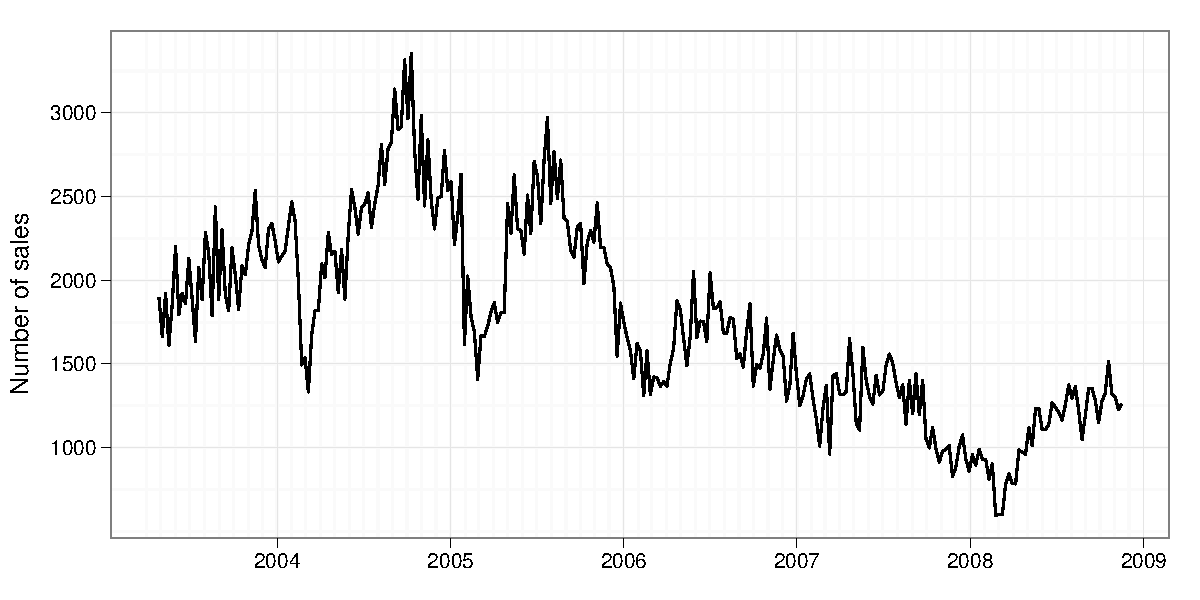
\includegraphics[width=0.5 \linewidth]{daily-sales}%
    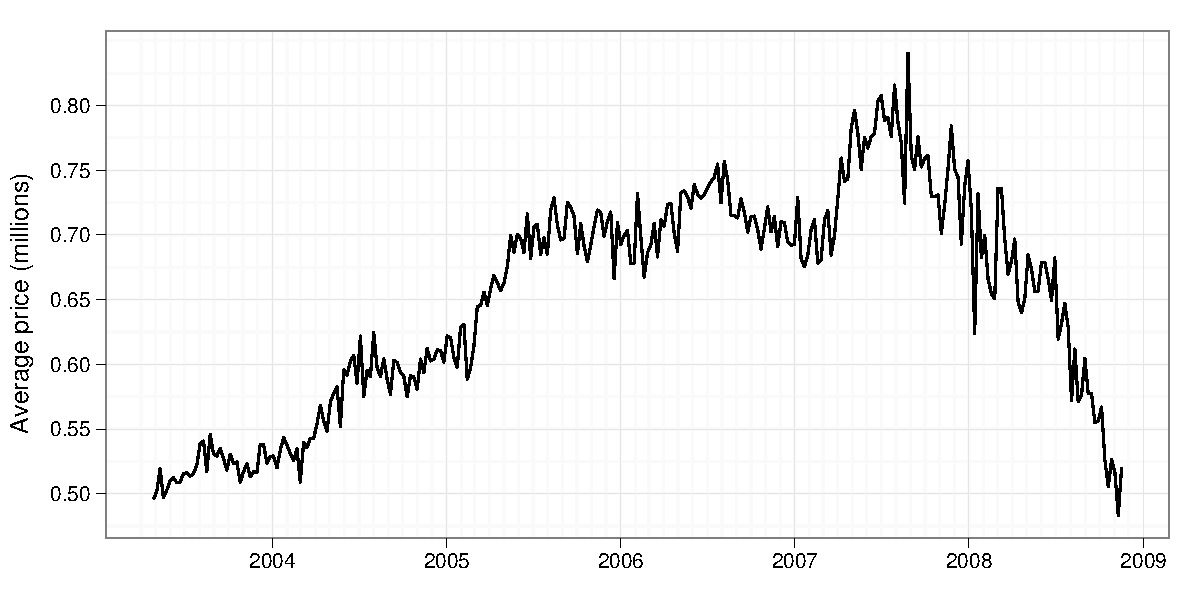
\includegraphics[width=0.5 \linewidth]{daily-price}%
  \caption{Weekly sales (left) and average prices (right).}
  \label{fig:daily}
\end{figure}

The data is over a relatively short period of time (6 years), but we might wonder if it's necessary to adjust for inflation, to ensure that the prices paid in 2003 are comparable to the prices paid today.

\subsection{Adjusting for inflation}
% explore-prices.r

A commonly used reference for determining inflation is the consumer price index ({\sc cpi}) produced by the Bureau of Labor Statistics, \url{http://www.bls.gov/CPI}.  The {\sc CPI} calculates the price of a weighted ``basket'' of frequently purchased consumer goods.  This price is calculated monthly, and we will use the West coast series, series CUUR0400SA0.
To adjust for inflation, we extract the data for the period data we have housing sales, and at for each month we calculate the ratio between the index at that time and at the end of 2008: we are adjusting all prices to 2008 prices. This is a common pattern in data analysis: we combine our original data with new data that provides context and helps us understand it better.  

% In this case, we want to control for changes in relative buying power (i.e.\ inflation).  Even over this relatively short time span it's a bad idea to ignore inflation: \$1\,000 2004 dollars would be worth\$1\,170 today.
% 

To show the effect of inflation, we index the CPI time series to the first date in the data.  This means we divide all of the values by the first value, converting the values into proportions.  This makes it easy to read the effect of inflation from the graph: a value of 1.1 represents a cumulative inflation of 10\% from the start of the data.  Indexing is a very useful technique and we'll use it throughout this analysis.  Figure~\ref{fig:inflation} shows the CPI-based inflation measurement and the affect of adjusting prices for inflation.  Inflation has been steadily climbing over the last five years, and failing to adjust for inflation makes the increasing trend prior to mid 2007 look more pronounced.  However, inflation adjustment is complicated because housing prices form a major part of the CPI, and because of this we chose not to inflation adjust the prices.

\begin{figure}[htbp]
  \centering
    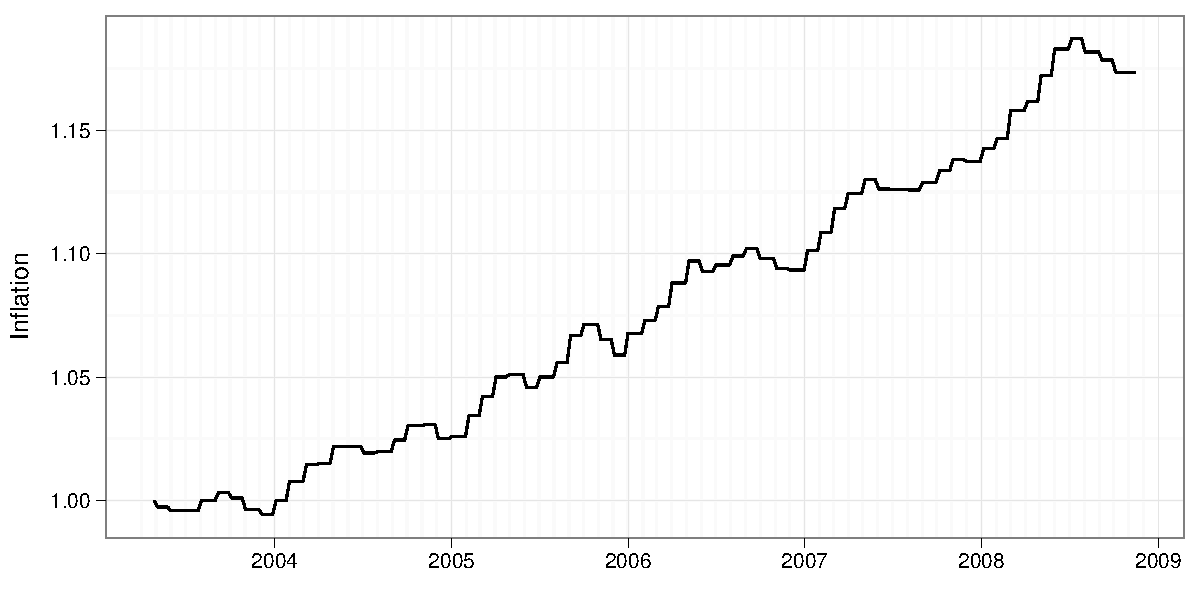
\includegraphics[width=0.5 \linewidth]{daily-cpi}%
    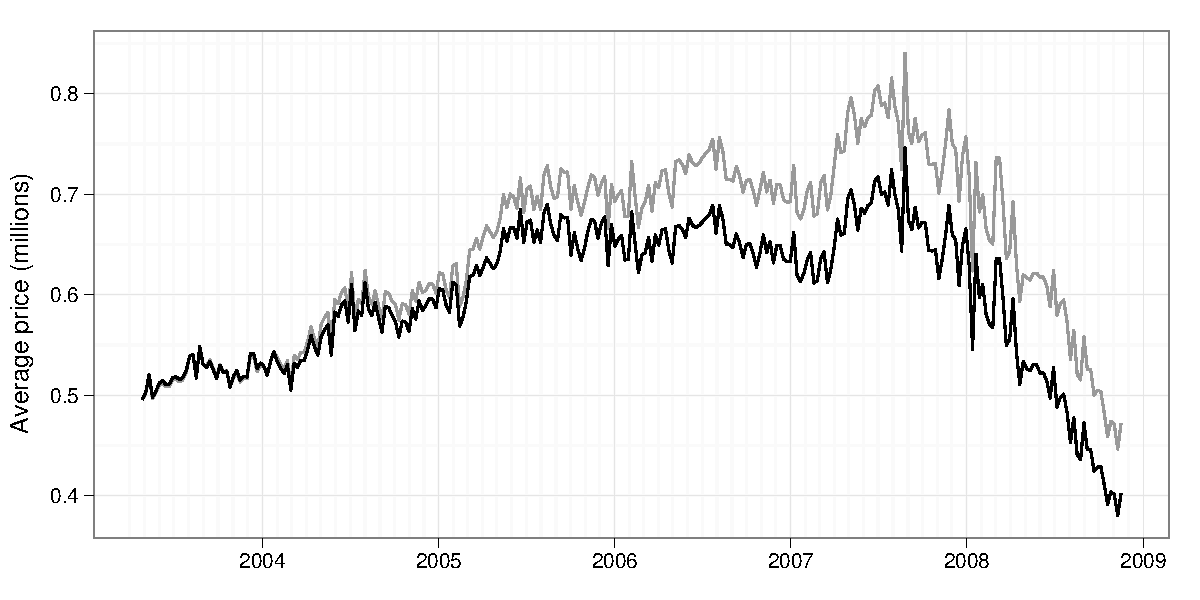
\includegraphics[width=0.5 \linewidth]{daily-price-adj}
  \caption{(Left) Inflation, indexed at 1 at start of series.  (Right) Inflation adjusted prices (black), and unadjusted prices (grey).  Failing to adjusting for inflation makes the rise look steeper, but has little effect on the decline.}
  \label{fig:inflation}
\end{figure}

With this basic overview in hand, it's time to start drilling into the details. In the following sections we break the house sales in to smaller groups, first by price and then by location.  We'll see whether the housing crisis has affected all equally, or some more than others.

\subsection{The rich get richer and the poor get poorer}
% explore-deciles.r

Has the housing crisis equally affected the rich and the poor?  Has the effect of the crisis been to improve or worsen the relative equality of these two groups?  In this section, we will explore how the crisis has effected the prices broken down by decile.  A big caveat is that we're looking at the Bay Area, so homes will be more expensive than many other places in the country, but we still might expect to see some relative inequalities.

To start our exploration, we calculate price deciles for each month.  The deciles are the nine prices that 10\%, 20\%, 30\%, 40\%, 50\%, 60\%, 70\%, 80\%, and 90\% of houses are cheaper than.  This is a succinct summary of the {\it distribution} of the prices for each month: instead of just looking at the average price, we are looking at nine numbers that summarise the complete distribution of the prices. 

Figure~\ref{fig:decile-raw} shows how these deciles have changed over time.  The top line is the ninth decile, the price that 90\% of houses are less than, and the bottom line is the first decile, the price that only 10\% of houses are cheaper than.  The line in the middle is the median, the price which divides the houses into halves, half cheaper and half more expensive.  The lines are coloured from dark to light from expensive to cheap.  Each line follows a similar pattern, and we can see the effect of the housing bubble in mid 2007, particularly in the most expensive houses.  

\begin{figure}[htbp]
  \centering
  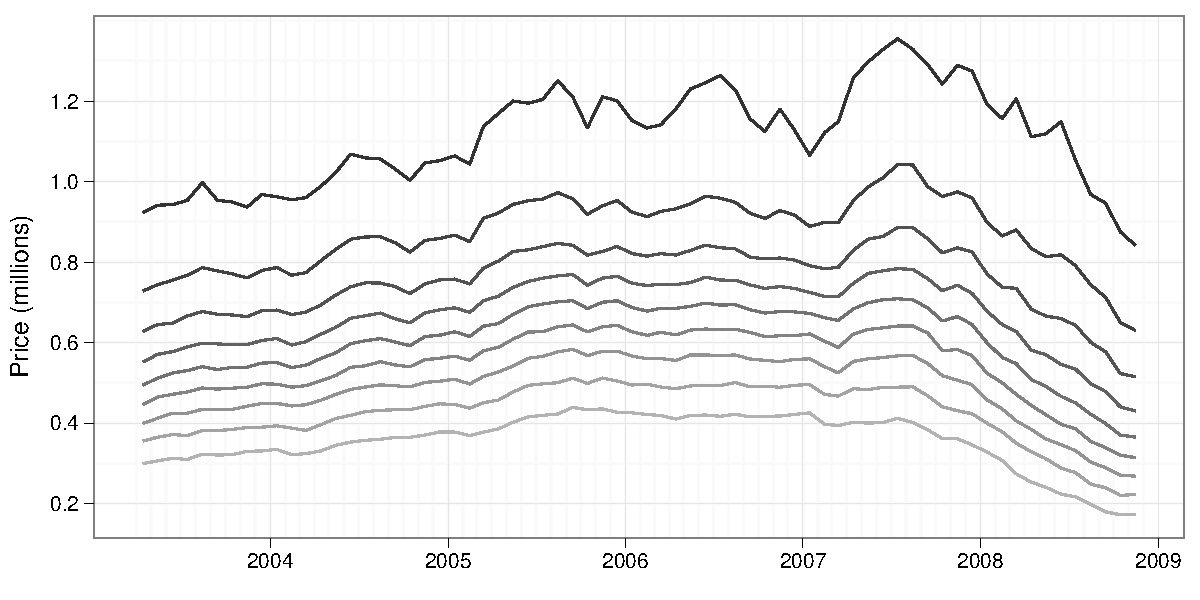
\includegraphics[width=0.75\linewidth]{decile-raw}
  \caption{Monthly average house price within each decile.  Cheaper houses (lower deciles) are coloured lighter.} 
  \label{fig:decile-raw}
\end{figure}

This plot lets us compare the absolute values of each decile, but maybe it is more appropriate to look at the relative prices: how have the prices changed proportionately.  One way to think about the relative price is to compare how each decile has changed from its starting value.  To do this we index each decile, just as we did for the {\sc cpi}. Figure~\ref{fig:decile-ind} shows these indices.  Each decile starts at one, and we can see the relative change in prices over time.  What's interesting in this plot is that the cheaper houses (the lighter coloured lines) seem to peak higher and earlier (mid 2005) than the most expensive houses, and then drop more rapidly.  The cheapest houses lost 43\% of their 2003 value compared to only 9\% for the most expensive houses.

\begin{figure}[htbp]
  \centering
  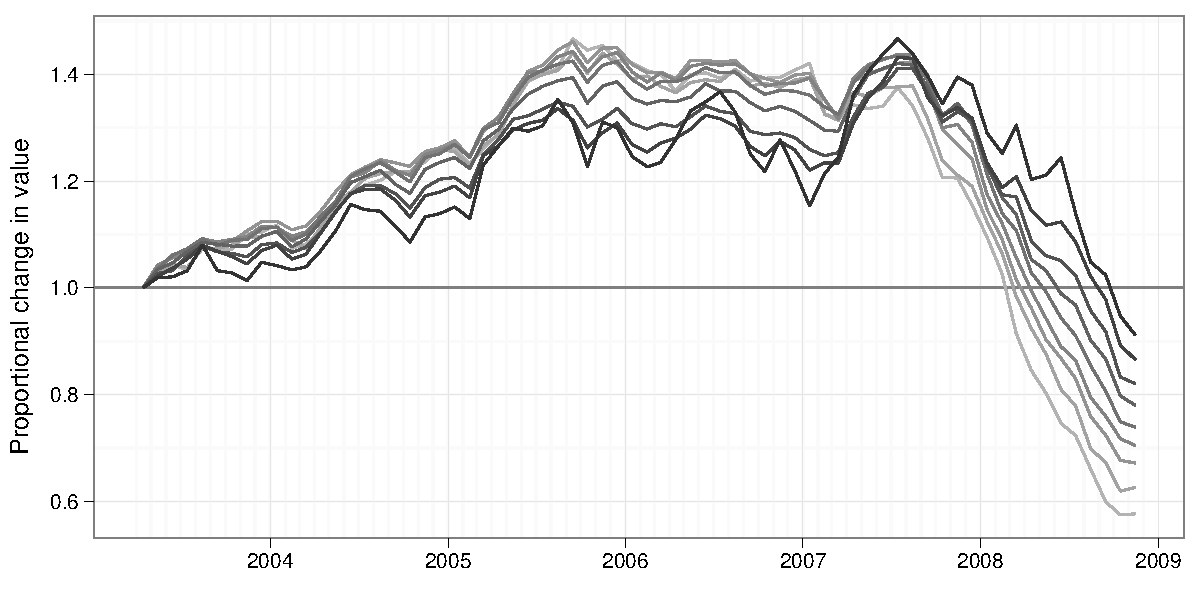
\includegraphics[width=0.75\linewidth]{decile-ind}
  \caption{Indexed house price within each decile.  The average price of cheaper houses peaked earlier and higher, and fell more steeply.}
  \label{fig:decile-ind}
\end{figure}

Another way to look at this inequality is Figure~\ref{fig:decile-rel}.  Here we have divided all the prices by the price of an average (median) home.  The values now represent a proportion of the median house price: a price of 1.2 represents a price 20\% higher than the median, and 0.8 20\% lower. Since the housing crisis, expensive houses have been getting relatively more expensive and cheap houses relatively cheaper.  One effect of the housing crisis has been to increase the difference between the cheapest and most expensive houses.

\begin{figure}[htbp]
  \centering
  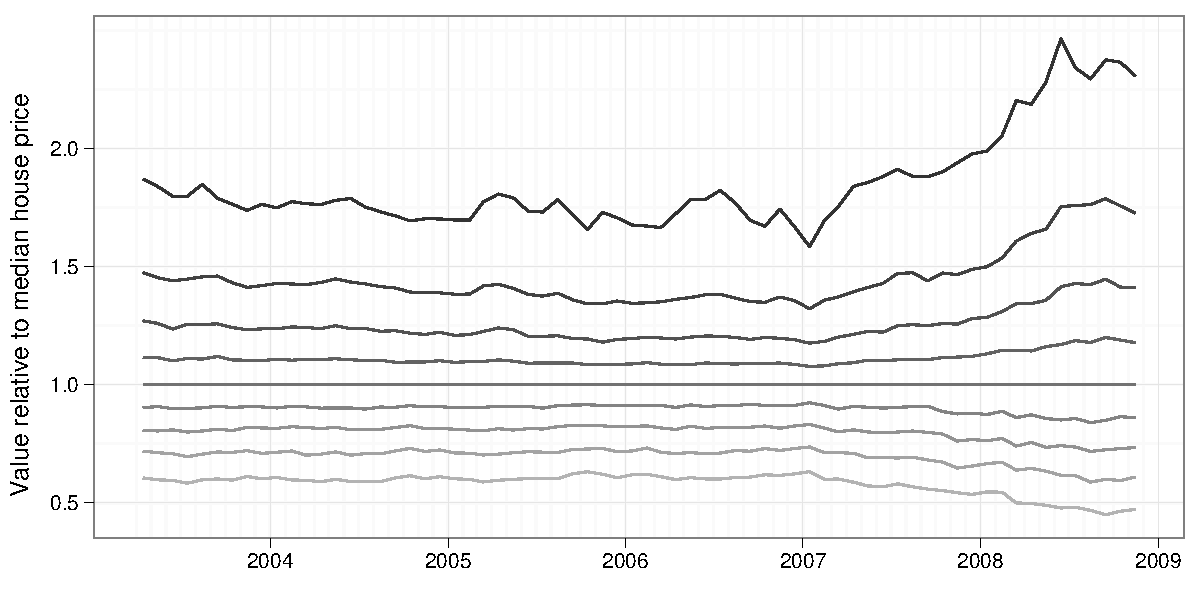
\includegraphics[width=0.75\linewidth]{decile-rel}
  \caption{House prices, relative to the price of the median priced home.  The disparity in home prices is increasing.}
  \label{fig:decile-rel}
\end{figure}

\subsection{Geographic differences}
% explore-city.r

We've just seen how the housing crisis has affected expense and cheap houses differently, but how does has it affected different cities?  In this section we'll explore how the effect of the housing crisis has varied over different cities in the bay area.  To do this, we'll need to first pick out all the cities that have a decent amount of data.  We decided to focus on all all cities with more than 2910 sales in total, an average of 10 sales per week.  This gives us 58 cities (of an original 245) with a total of 428,415 sales (out of an original 521,726, 82\%).  

From this data we then calculated the average house price for each city for each week.  Figure~\ref{fig:spaghetti} shows this data, with each city as a different line.  Statisticians have an evocative name for this type of plot: the spaghetti plot.  It's very hard to see anything in the big jumble of lines.  One way to improve this is to smooth each line, to to focus on the overall trend, removing short-term variation that we're not so interested in. 

\begin{figure}[htbp]
  \centering
    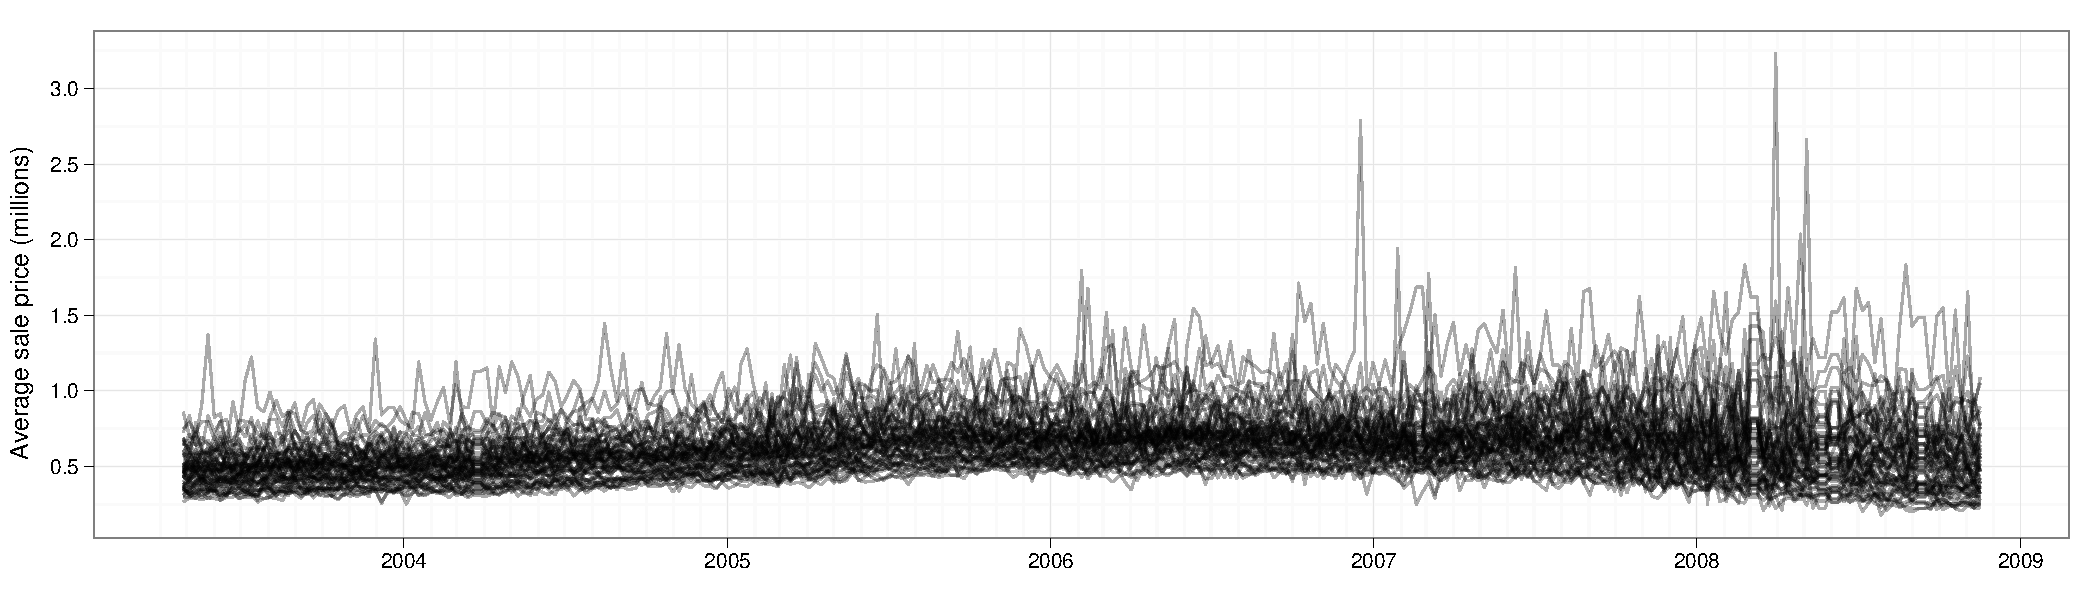
\includegraphics[width=0.9\linewidth]{cities-price}
  \caption{Average sale price for each week for each city.  This type of plot is often called a spaghetti plot.}
  \label{fig:spaghetti}
\end{figure}

There are many different ways to create smooth curves, and our purposes of them most of them are fine.  We used generalised additive models ({\sc gam}) are a generalisation of linear models \citep{wood:2006}, which by finding the optimum trade-off between fitting the data and minimising the wiggliness of the line.  The effect is to remove noisy short-term effects and focus on the long-term trend.  This is what we want: we're not interested in daily or weekly changes, we're interested in the long-term changes related to the housing crisis.

The left part of Figure~\ref{fig:smoothed} shows the the result of this smoothing. This is a big improvement and we can now actually see some patterns! Note the big difference in scales between this plot and the first: smoothing the data has removed the large spikes which represent the sales of few very expensive houses. We'll also index each city like we indexed each decile: dividing out the starting price puts each city onto an common scale and allows us to focus on the changes.

\begin{figure}[htbp]
  \centering
  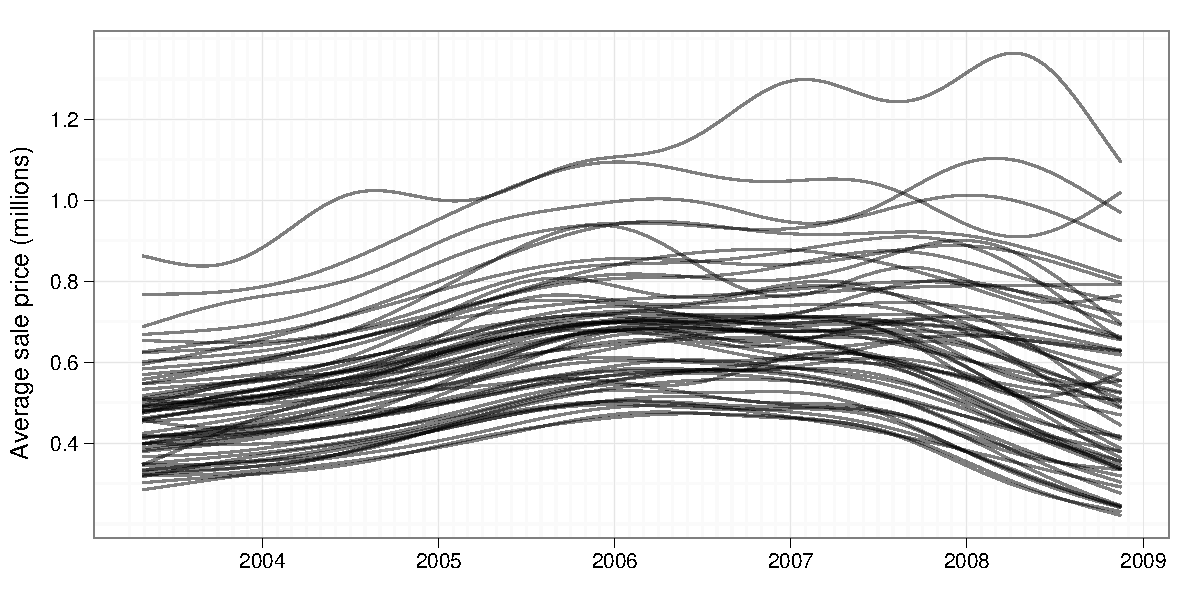
\includegraphics[width=0.5 \linewidth]{cities-smooth}%
  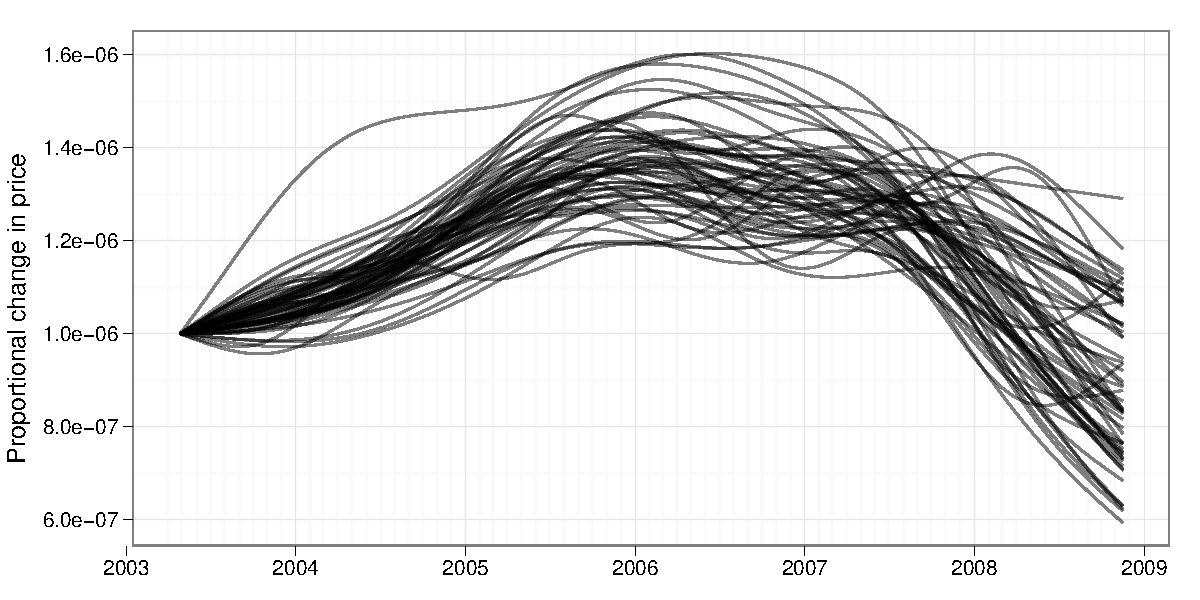
\includegraphics[width=0.5 \linewidth]{cities-indexed}
  \caption{Smoothed city-level weekly average sale prices.  Compared to the non-smoothed version it's easier to see the long-term trends, but it's still not particularly easy.}
  \label{fig:smoothed}
\end{figure}

There are still a lot of the lines in that plot and we might be missing important findings, so instead of displaying all the cities in plot, we looked at each city individually, as in Figure~\ref{fig:individual}.  This takes up a lot of room, but if you have a big screen or a good printer it's really worthwhile.  We can pick out some interesting patterns: Berkeley and San Francisco show less of a peak and less of a drop, and Mountain View seems not all affected by the crisis.  Other cities, like Oakley, Vallejo, and San Pablo, show big peaks and big drops: 



% Figure~\ref{fig:clustering} shows one way of clustering the cities into three groups.  Note how the groups are basically formed along the diagonal: it's the difference between the peak and the plummet that seems to be telling us the most.  Figure~\ref{fig:clustered} shows the result of the clustering, with each of the three groups displayed in its own panel.  The groups are somewhat arbitrary (we could shift the boundaries a little in either direction and have little effect)
% 
% \begin{figure}[htbp]
%   \centering
%     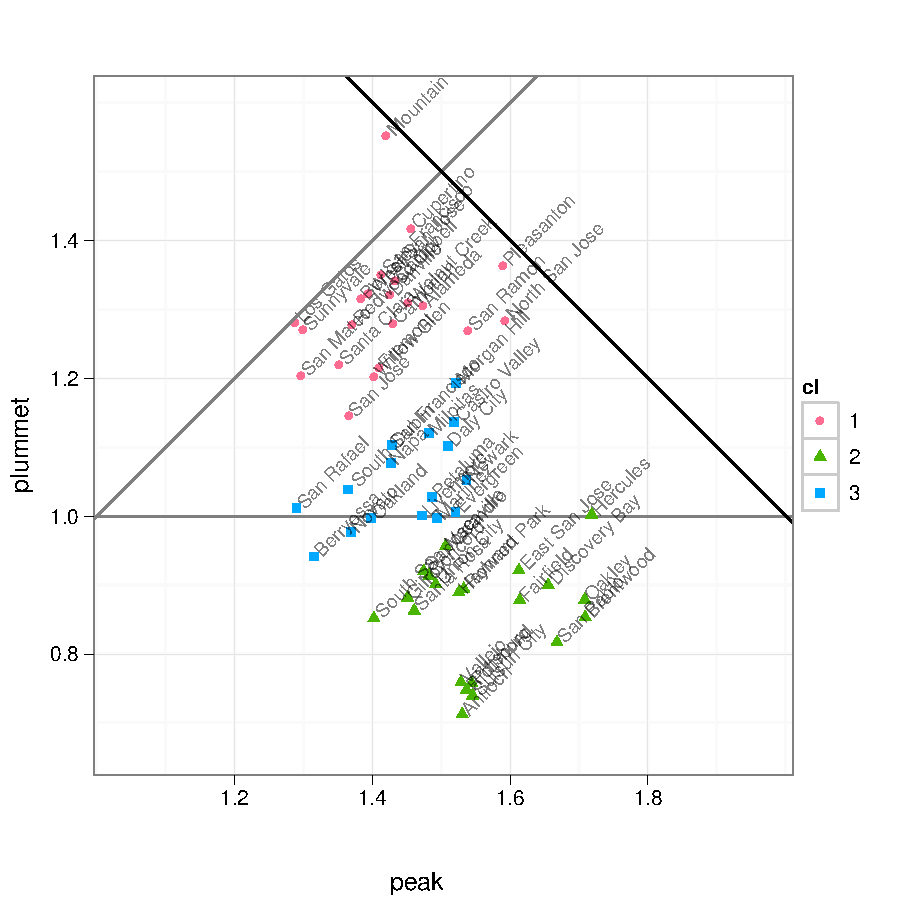
\includegraphics[width=0.7 \linewidth]{cities-clustering}
%   \caption{A scatterplot of cities with height at peak on x axis, and most recent value (plummet) on y axis.  The cities have been clustered into three groups.  The closer a city is to the line in the top left corner, the less the effect of the housing crisis on average prices.}
%   \label{fig:clustering}
% \end{figure}
% 
% \begin{figure}[htbp]
%   \centering
%   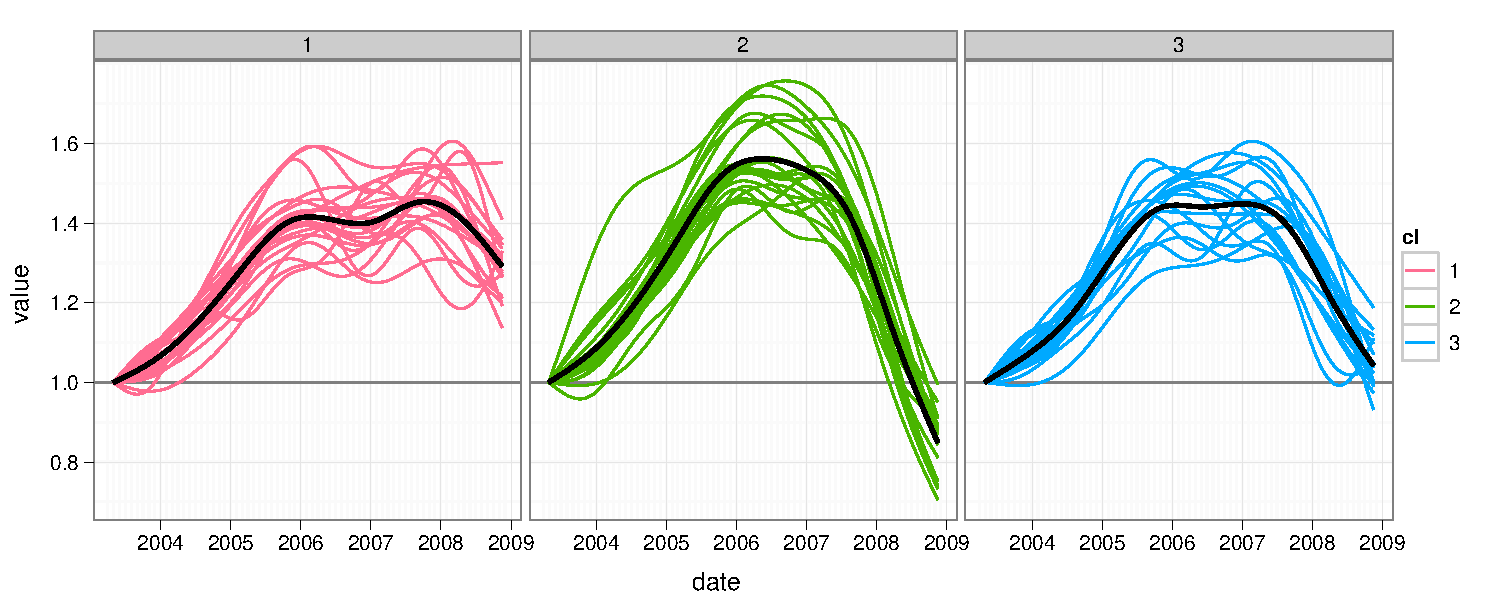
\includegraphics[width=\linewidth]{cities-indexed-clustered}
%   \caption{The index sale price time series for the three clustered identified in Figure~\ref{fig:clustering}.  Cluster one includes cities with low peak and no plummet, cluster two cities with high peak and big plummet, and cluster three is somewhere in between.  The thick lines represent smoothed patterns within each cluster.}
%   \label{fig:clustered}
% \end{figure}

After a few false starts we realised that there was one main feature that seemed to distinguish the different cities: difference between prices at the peak of the boom and the depth of their most recent plummet.  Figure~\ref{fig:groups} groups the cities by the value of this new variable.  The divisions are arbitrary, but you can see how the cities in each group follow a similar pattern.  This supports our view that this single number is a good summary for the effect of the housing crisis.

\begin{figure}[htbp]
  \centering
    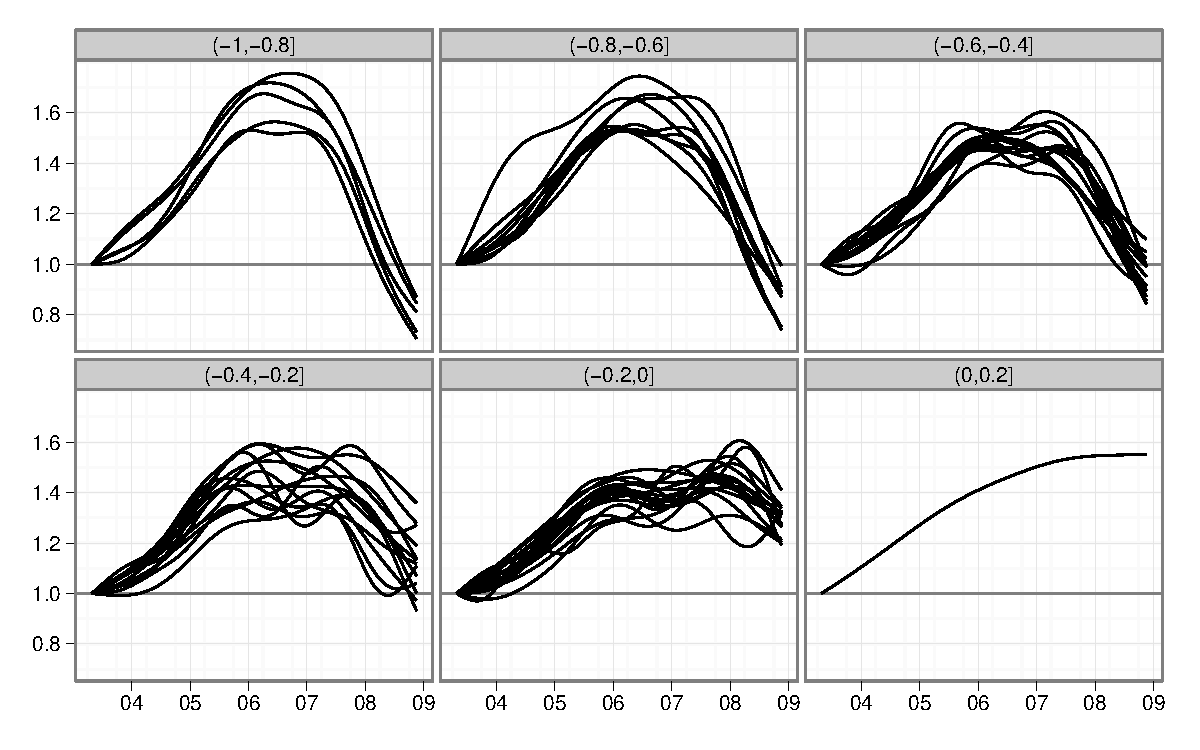
\includegraphics[width=0.75\linewidth]{cities-indexed-grouped}
  \caption{A separate plot for each 0.2 interval drop.  The patterns within each group are similar, suggesting that this one number does a good job of  }
  \label{fig:groups}
\end{figure}

We have determined that some cities showed a different pattern to others, but why? Plotting the geographic pattern, as in Figure~\ref{fig:geo} doesn't reveal anything particularly striking except that the worst hit towns tend to be the north and the east. This doesn't offer much in the way of explanatory power, so we looked for other variables that might help us to understand what's going on. 

\begin{figure}[htbp]
  \centering
    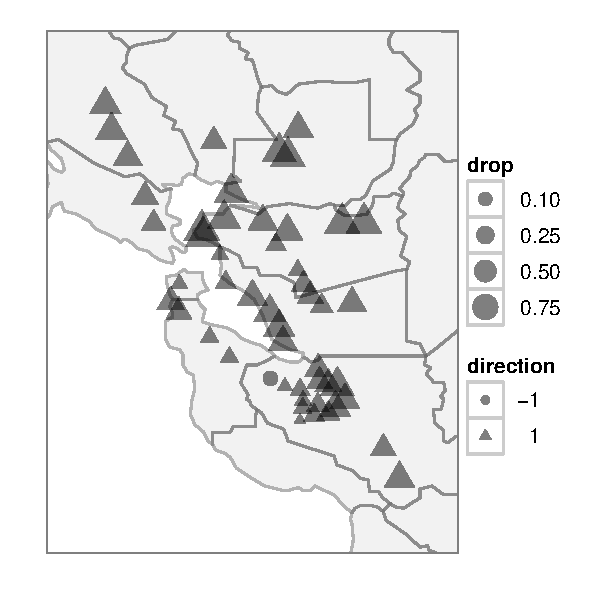
\includegraphics[width=0.4\linewidth]{cities-geo-changes}
  \caption{The geographic distribution of price drops.}
  \label{fig:geo}
\end{figure}

The census quickfacts site, e.g.\ \url{http://quickfacts.census.gov/qfd/states/06/0649670.html}, provides a number of interesting demographic variables for each city.  Unfortunately the data isn't available in an easily downloadable format, so we had to resort to another set of scripts to scrape the data and convert it into csv.  There were also some differences in what constituted a city in the census data and so we could only match 46 out of the full 58 cities.  The cities that weren't matched were either too small, or included in a large city in the census data.

\begin{figure}[htbp]
  \centering
  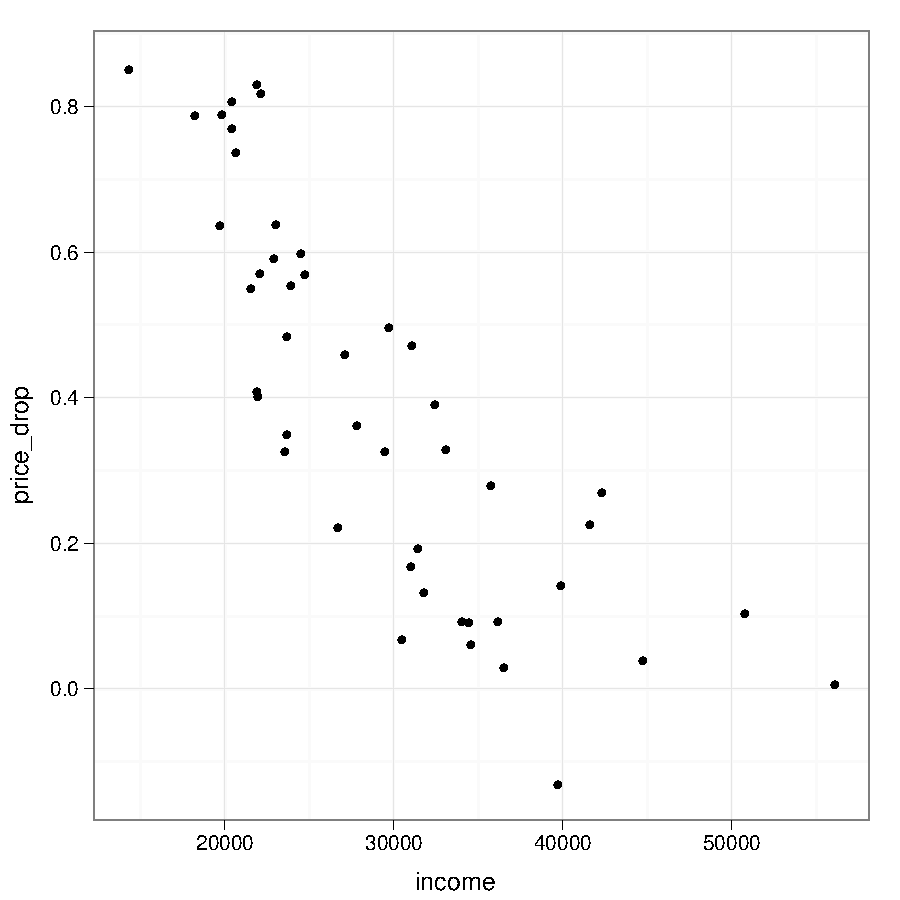
\includegraphics[width=0.33\linewidth]{cities-income}%
  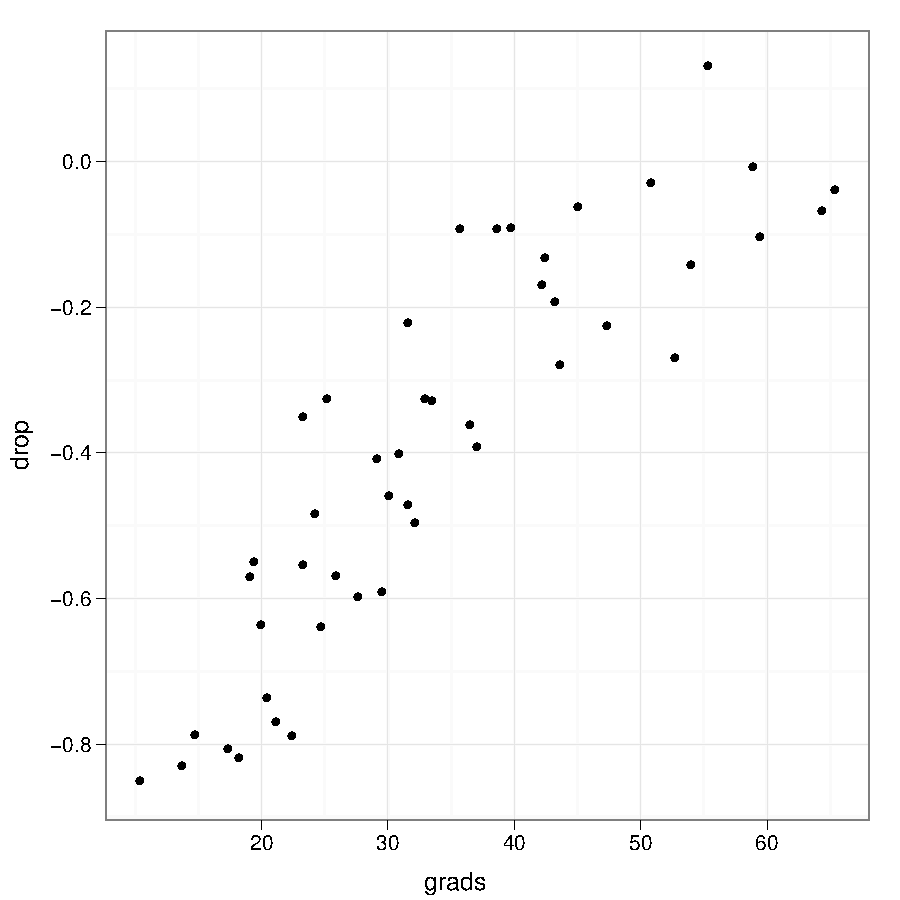
\includegraphics[width=0.33\linewidth]{cities-grads}%
  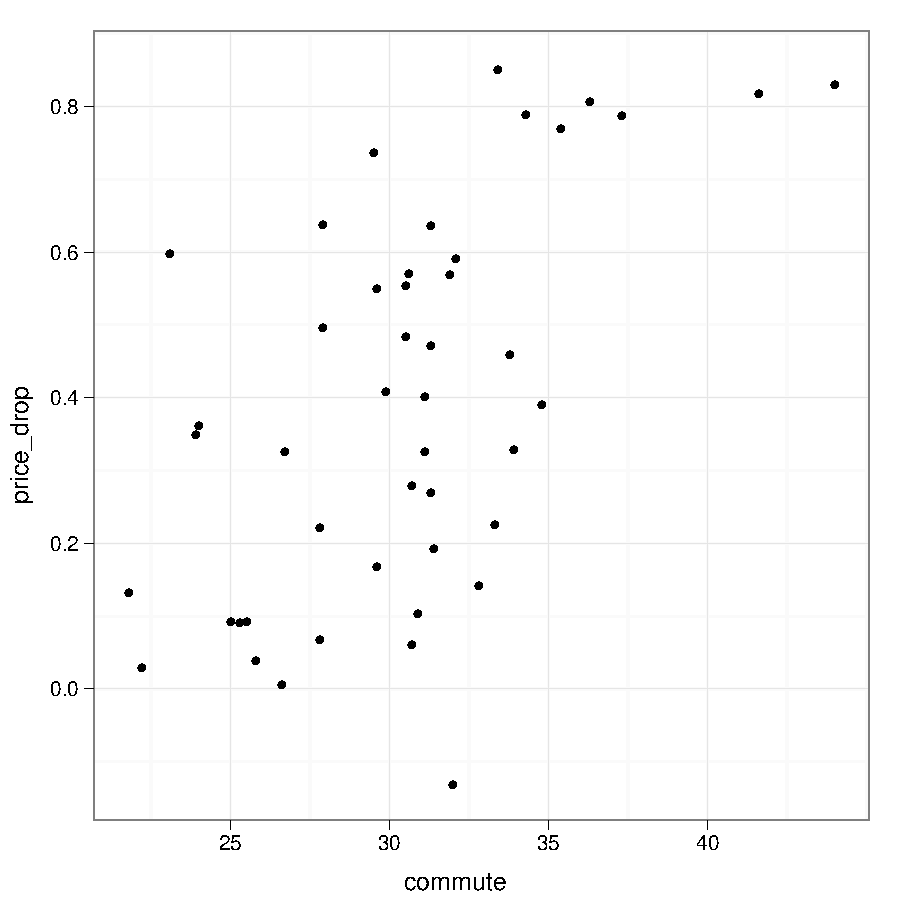
\includegraphics[width=0.33\linewidth]{cities-commute}
  
  \caption{From left to right, the relationship between the drop in house prices and average income, percent of college graduates and average commute time.}
  \label{fig:census}
\end{figure}

Looking at these variables revealed the following interesting relationships.  The most affected cities have a high percentage of  babies and children, bigger households, fewer bachelors degrees, and longer commutes.  Most significantly these cities also have lower incomes, which is probably the factor that drives all of the other relationships. Figure~\ref{fig:census} shows three scatterplots showing the relationship between the drop and income, percent of college graduates and commute time.  The relationship with commute time is weak, but striking in that all of the cities with particularly long commute times have particularly large drops.  It appears that the housing crisis  has been relatively more damaging to the house prices of people who live in poorer areas.

\begin{figure}[htbp]
  \centering
  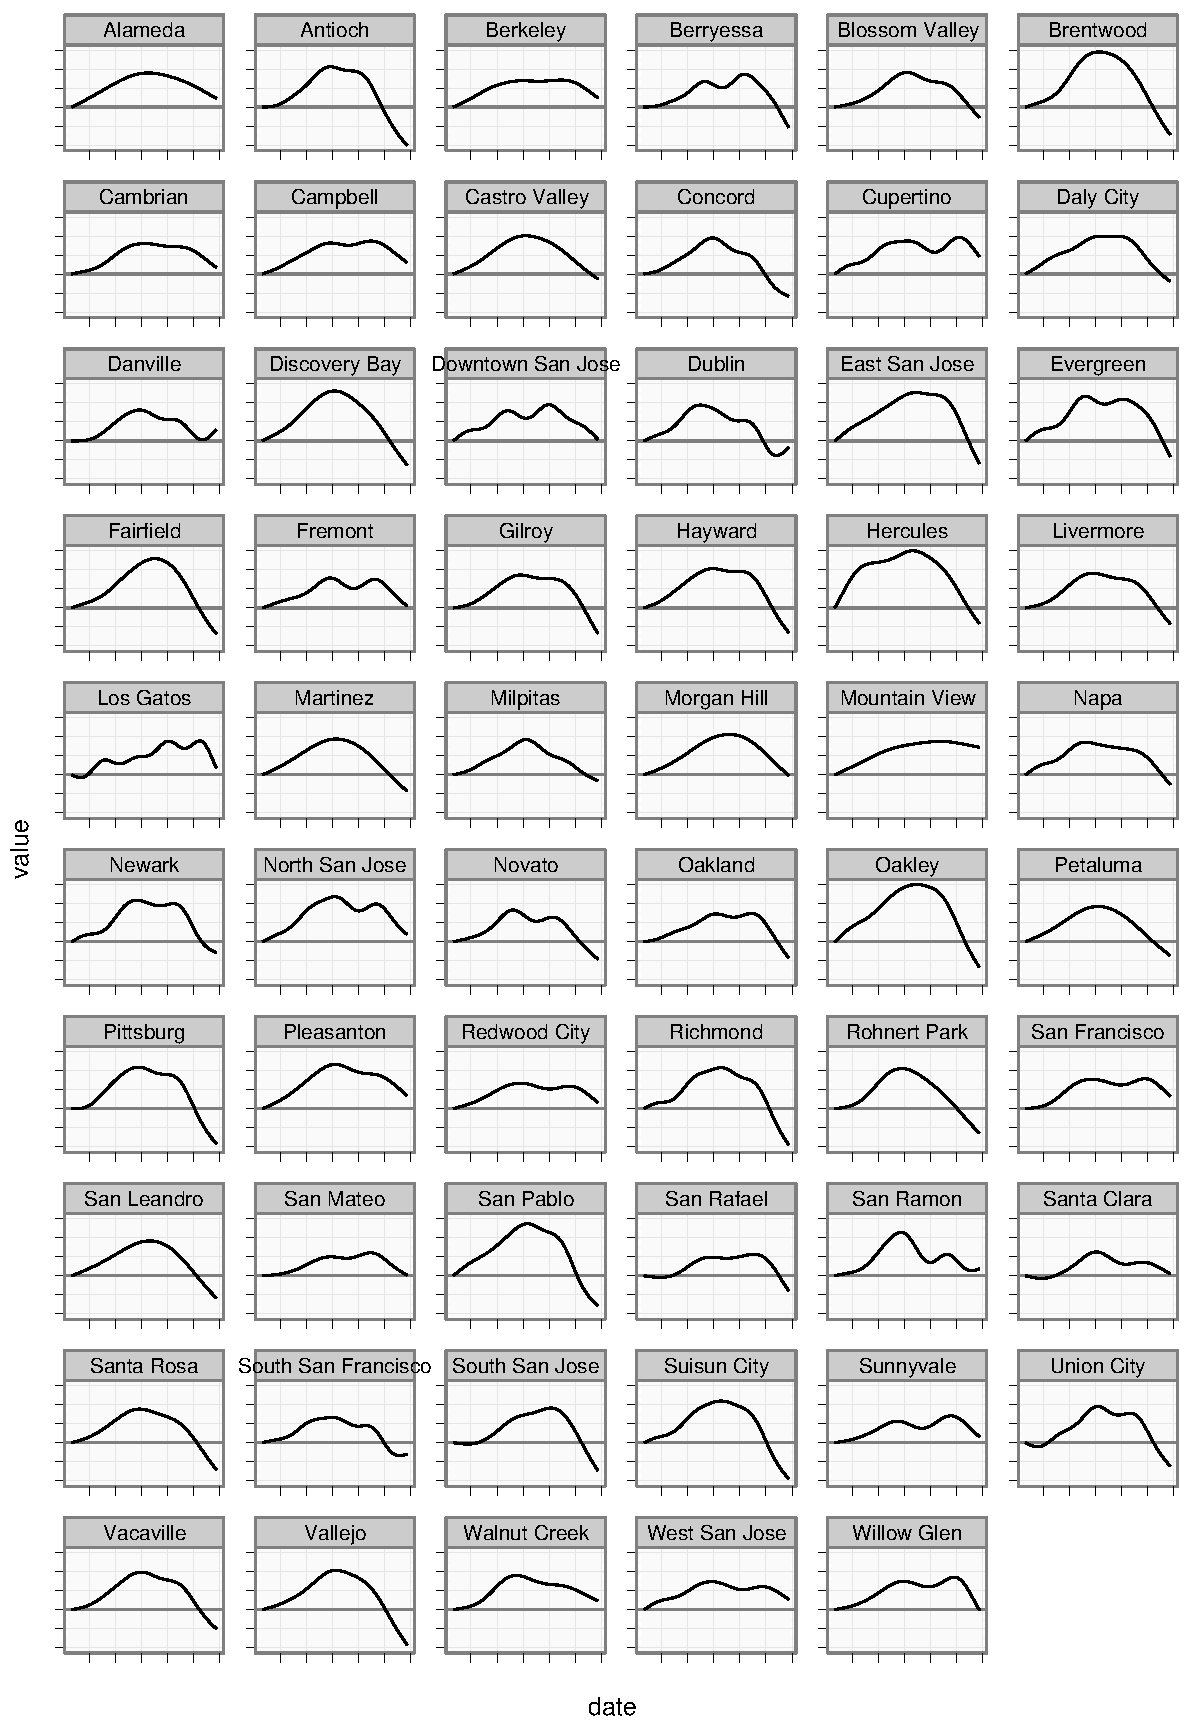
\includegraphics[width=0.9\linewidth]{cities-individual}
  \caption{Individual plots for each city.}
  \label{fig:individual}
\end{figure}

\section{Exploring San Francisco}

Having explored the difference between cities, we turned to look at a single city in more detail.  We chose San Francisco because it's the city that collectively we were most familiar with, and it has some iconic features that it should be easy for others to identify as well.  We started our exploration by extracting all addresses within San Francisco that were geocoded to block interpolation or better, giving us a total of 25,377 addresses.  We this data we did a very simple plot: a scatterplot of the latitudes and longitudes, Figure~\ref{fig:sf-geo}.  For the residential parts of SF, this gives an amazingly detailed picture.  We can see Golden Gate and San Bruno parks, but our view of downtown is patchy, because there are few residential homes there.

\begin{figure}[htbp]
  \centering
  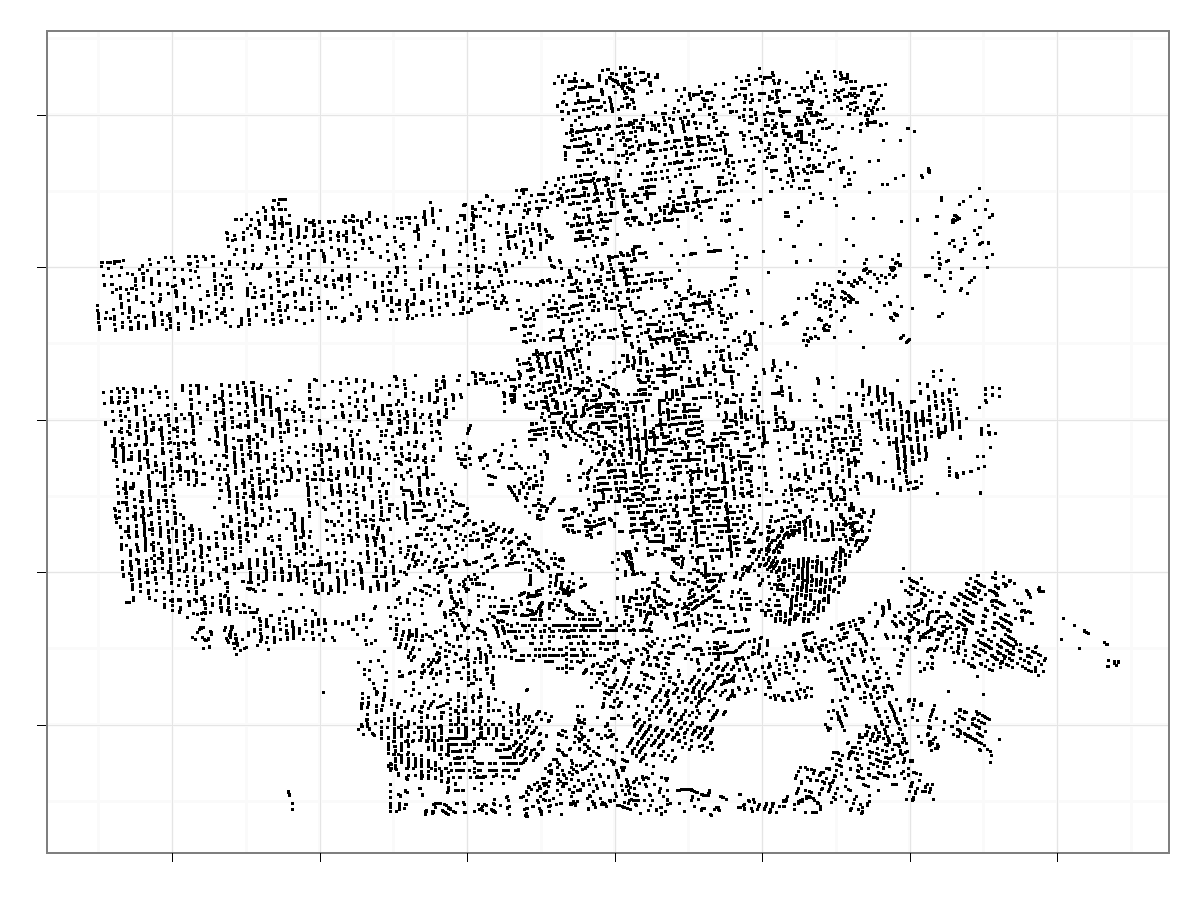
\includegraphics[height=2in]{sf-geo}%
  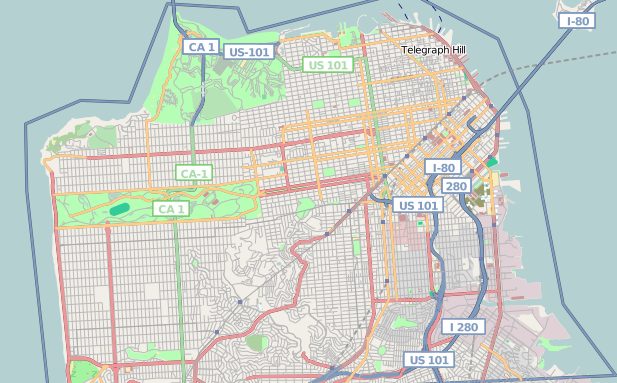
\includegraphics[height=2in]{sf-map}
  \caption{(Right) map of San Francisco from \url{http://openstreetmap.com}}
  \label{fig:sf-geo}
\end{figure}

One problem with this plot is we lose all feel for how many sales are in each location.  Figure~\ref{sf-n} shows two attempts to recapture the information.  On the left, we have a bubbleplot with the size of the location proportional to the number of sales.  We now get quite a different view of the downtown: there are very large number of sales down there.  Looking closer at the data reveals that these are apartment buildings with hundreds of apartments.  On the right, we have divided SF in to squares of 0.005 latitude and longitude and counted the number of houses in each bin.  This gives us higher level view of where the houses are and will be useful for the next step, exploring how prices vary geographically within the city.

\begin{figure}[htbp]
  \centering
    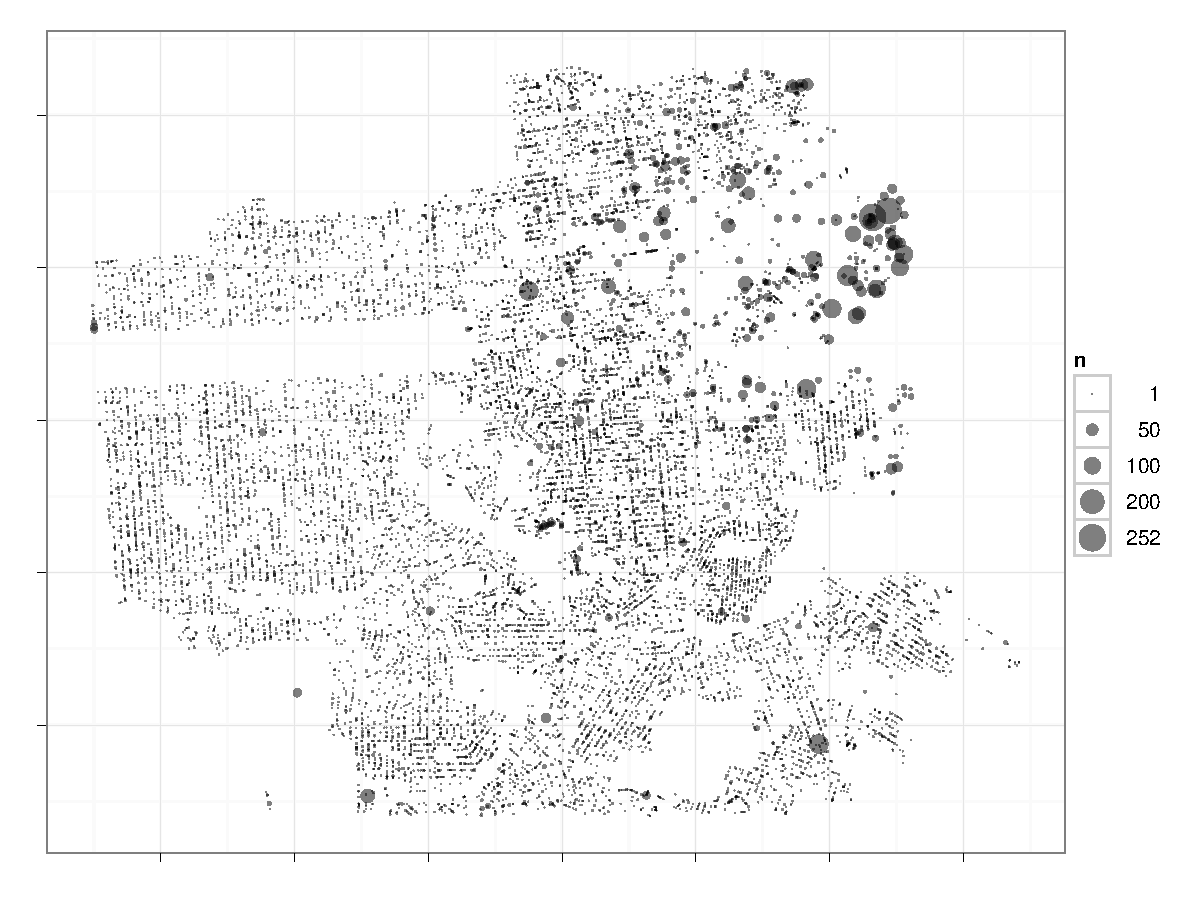
\includegraphics[width=0.5\linewidth]{sf-geo-n}%
    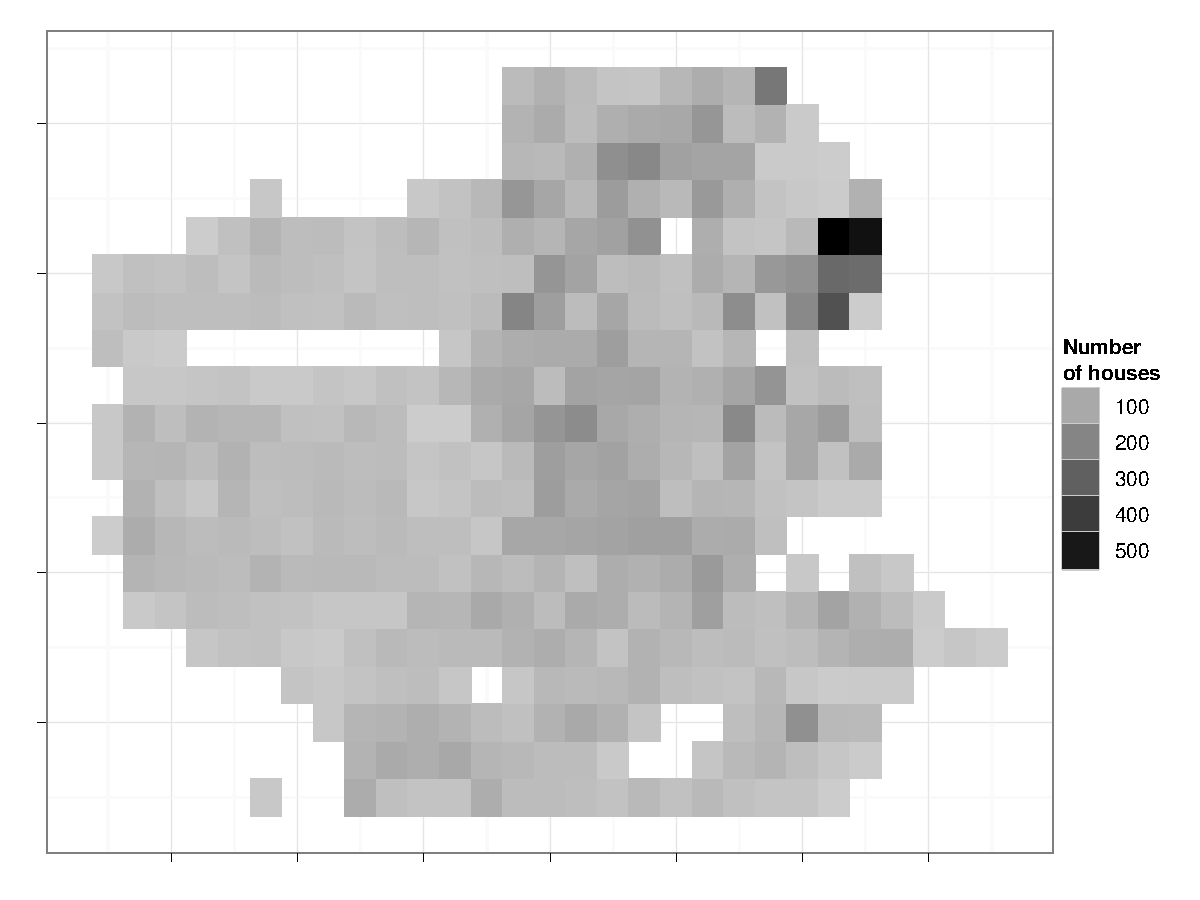
\includegraphics[width=0.5\linewidth]{sf-bin-n}
    % 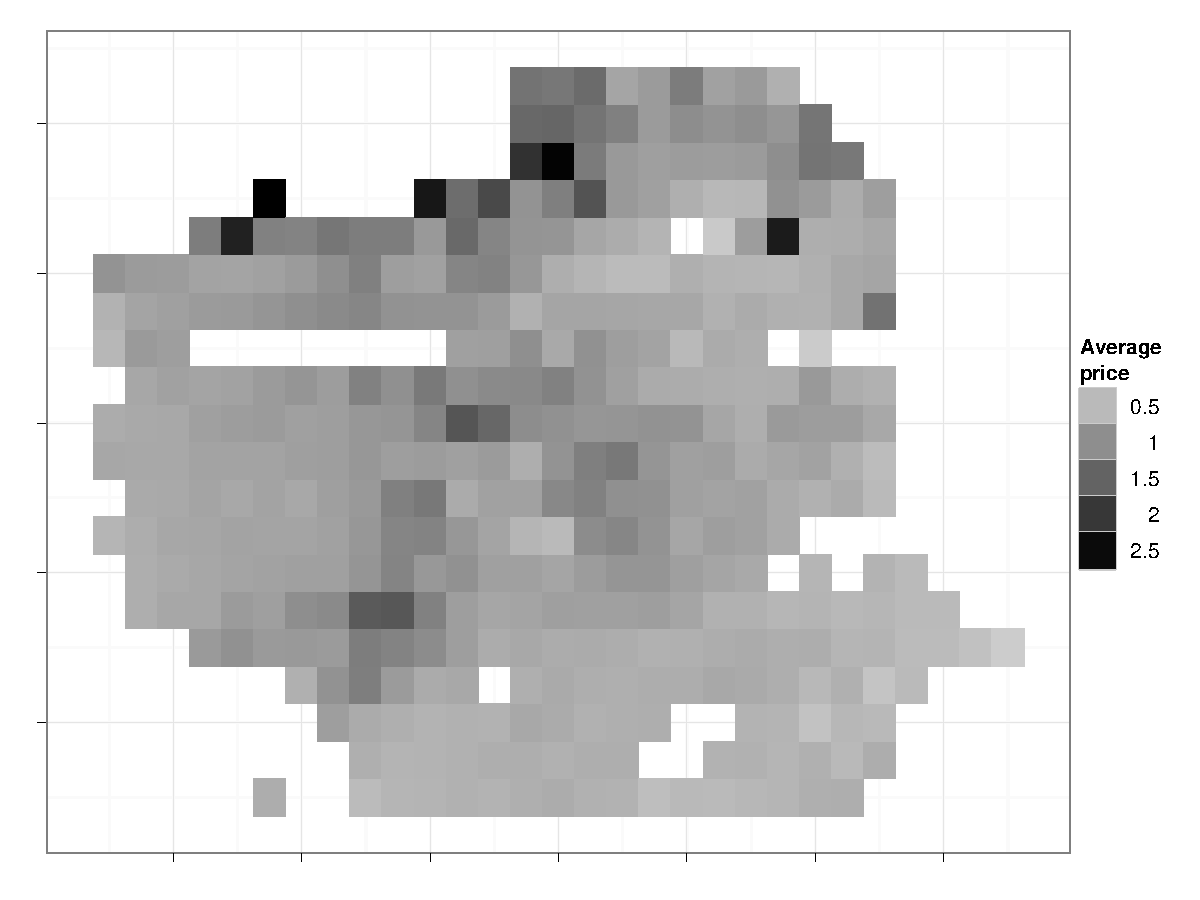
\includegraphics[width=0.5\linewidth]{sf-bin-price}
    % 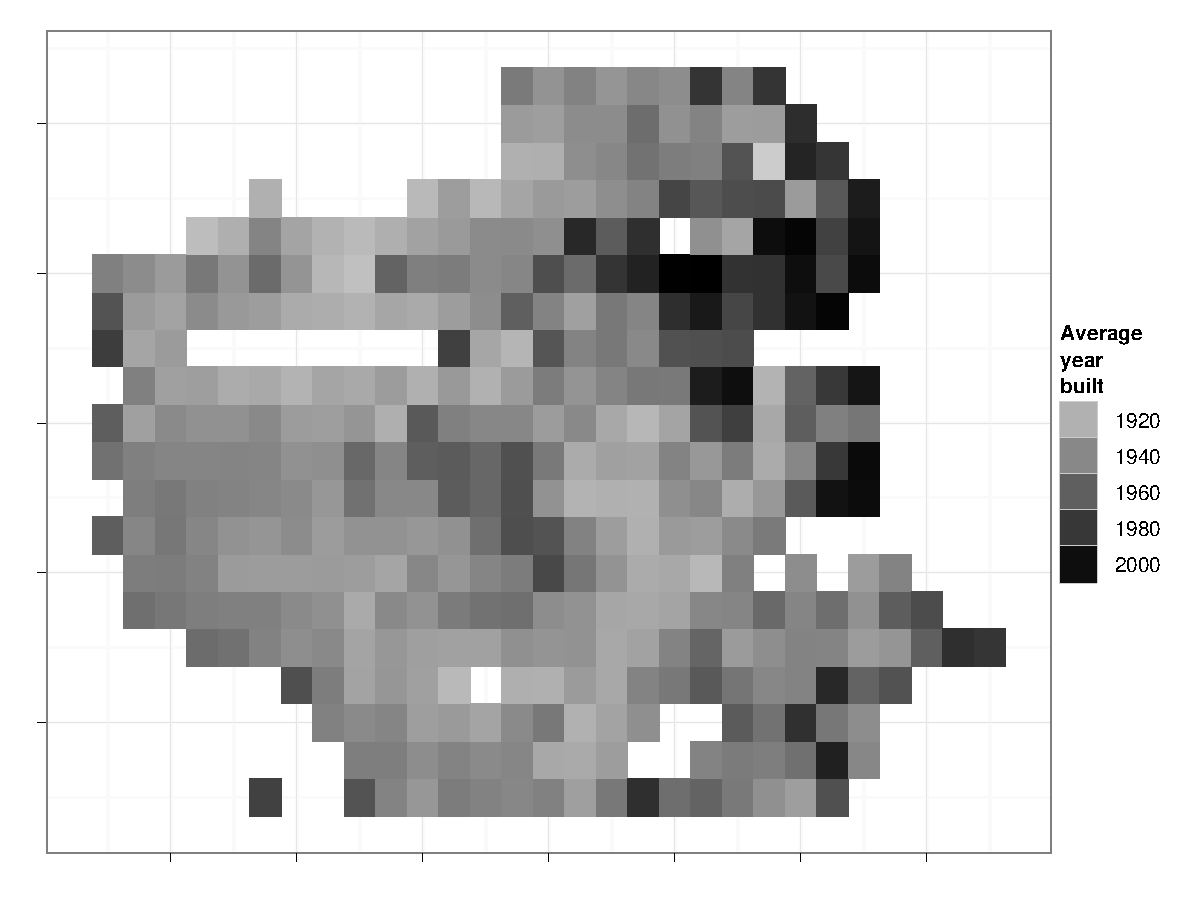
\includegraphics[width=0.5\linewidth]{sf-bin-built}%
    % 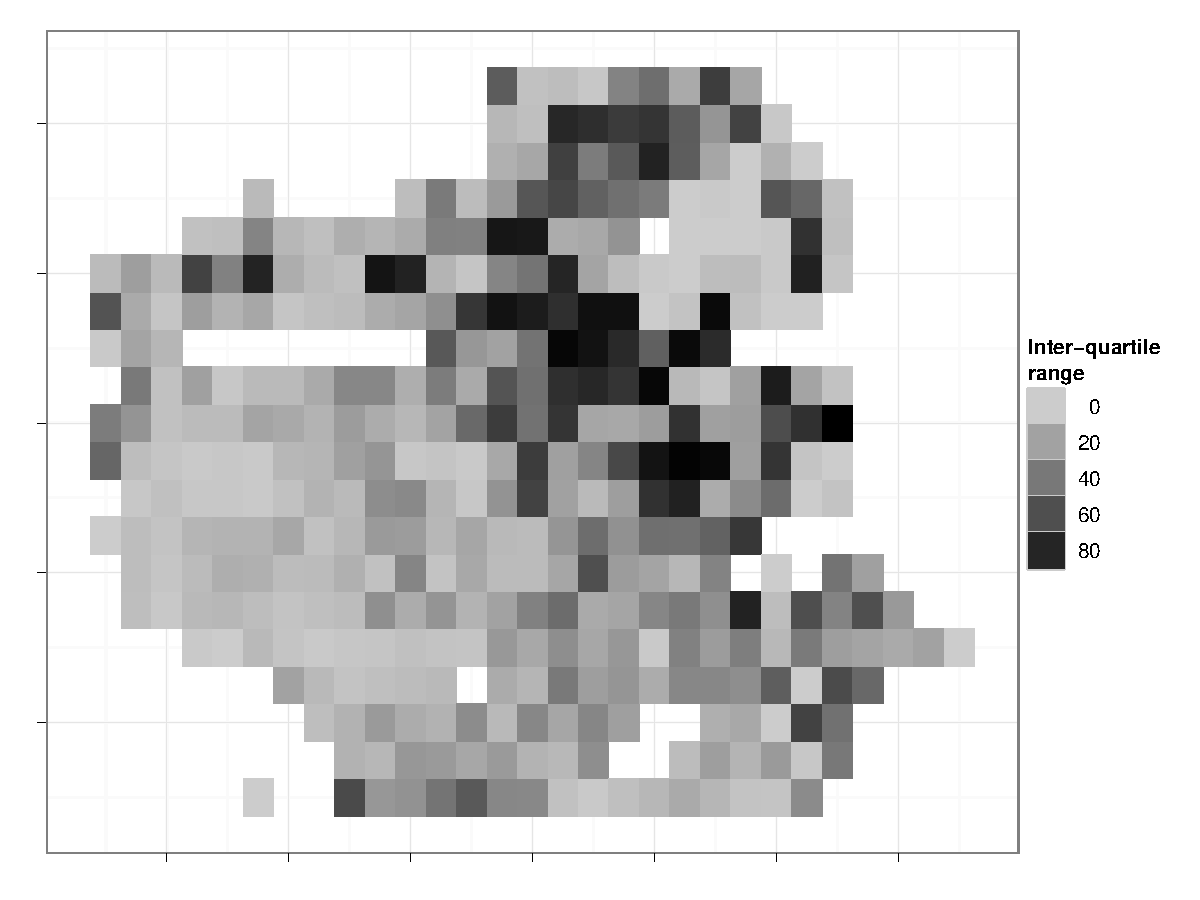
\includegraphics[width=0.5\linewidth]{sf-bin-iqr}
  \caption{caption}
  \label{fig:sf-n}
\end{figure}

Using that same binning, we calculate the house price deciles.  Figure~\ref{sf-price} shows the geographic distribution of two functions of the deciles.  On left we display the median house price for each bin.  We can see the most expensive houses border the Presidio and coast to the North of SF.  The number displayed on the right is a little more complicated to explain - it's the difference between the first and ninth deciles, divided by the median.  This is a measure of relative variation (a analogue to the coefficient of variation), giving the number of median house prices between the cheapest and most expensive houses.

\begin{figure}[htbp]
  \centering
    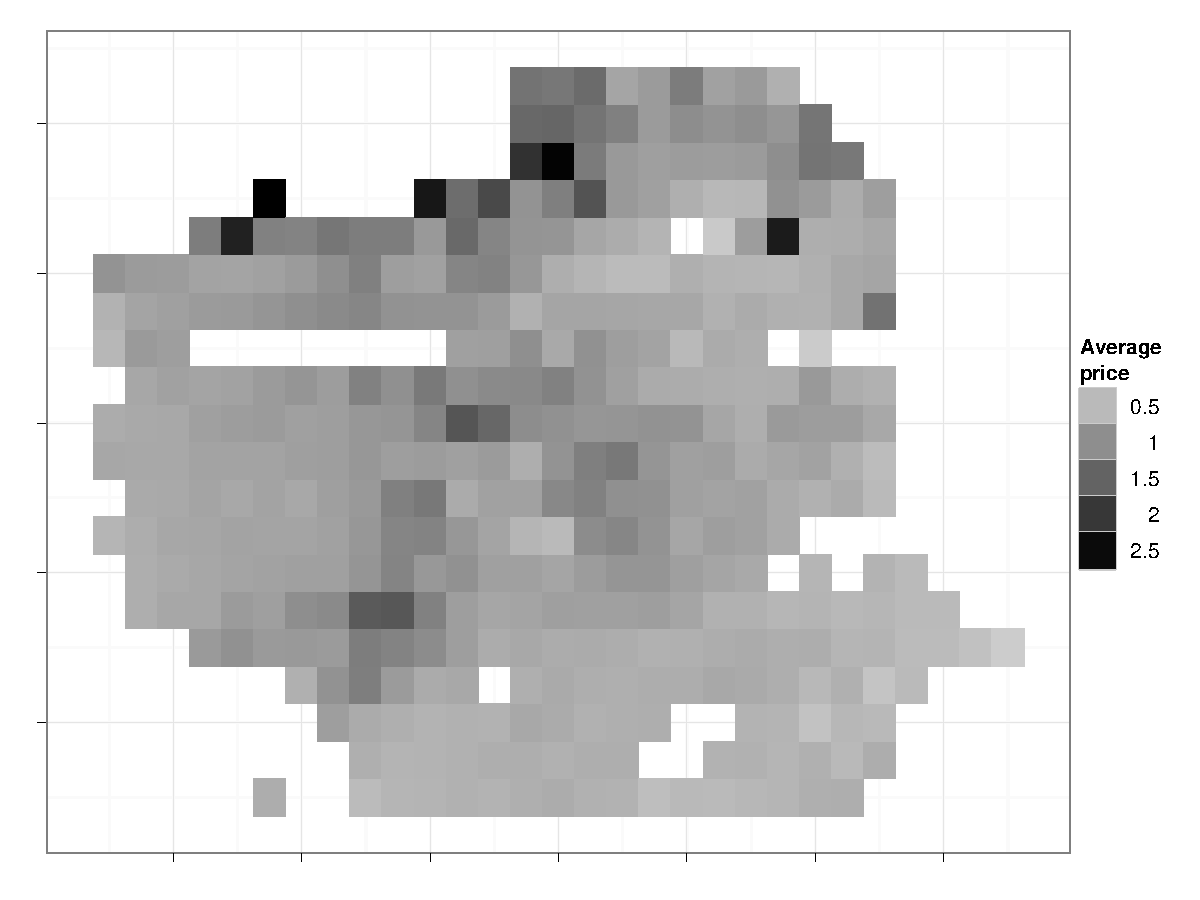
\includegraphics[width=0.5\linewidth]{sf-bin-price}%
    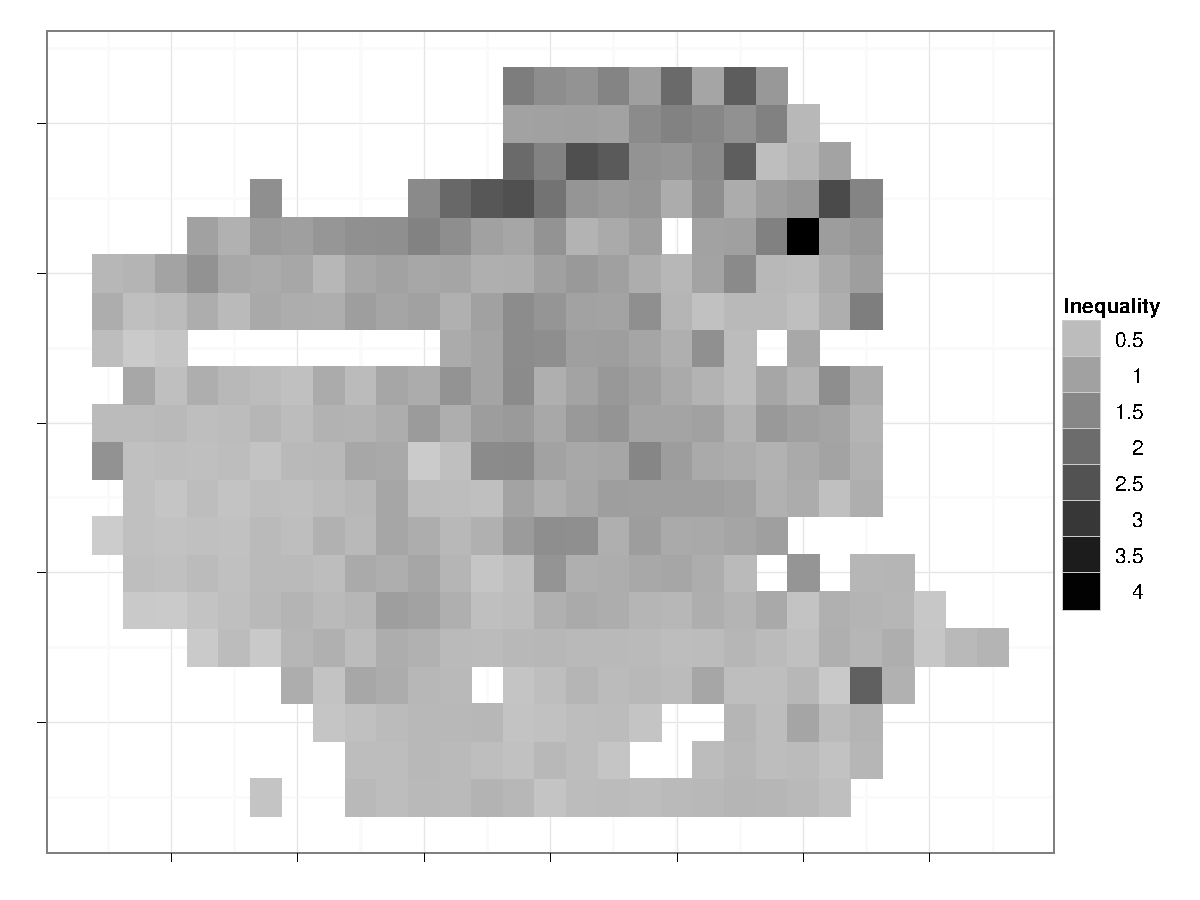
\includegraphics[width=0.5\linewidth]{sf-bin-ineq}
  \caption{caption}
  \label{fig:sf-price}
\end{figure}

% \begin{figure}[htbp]
%   \centering
%   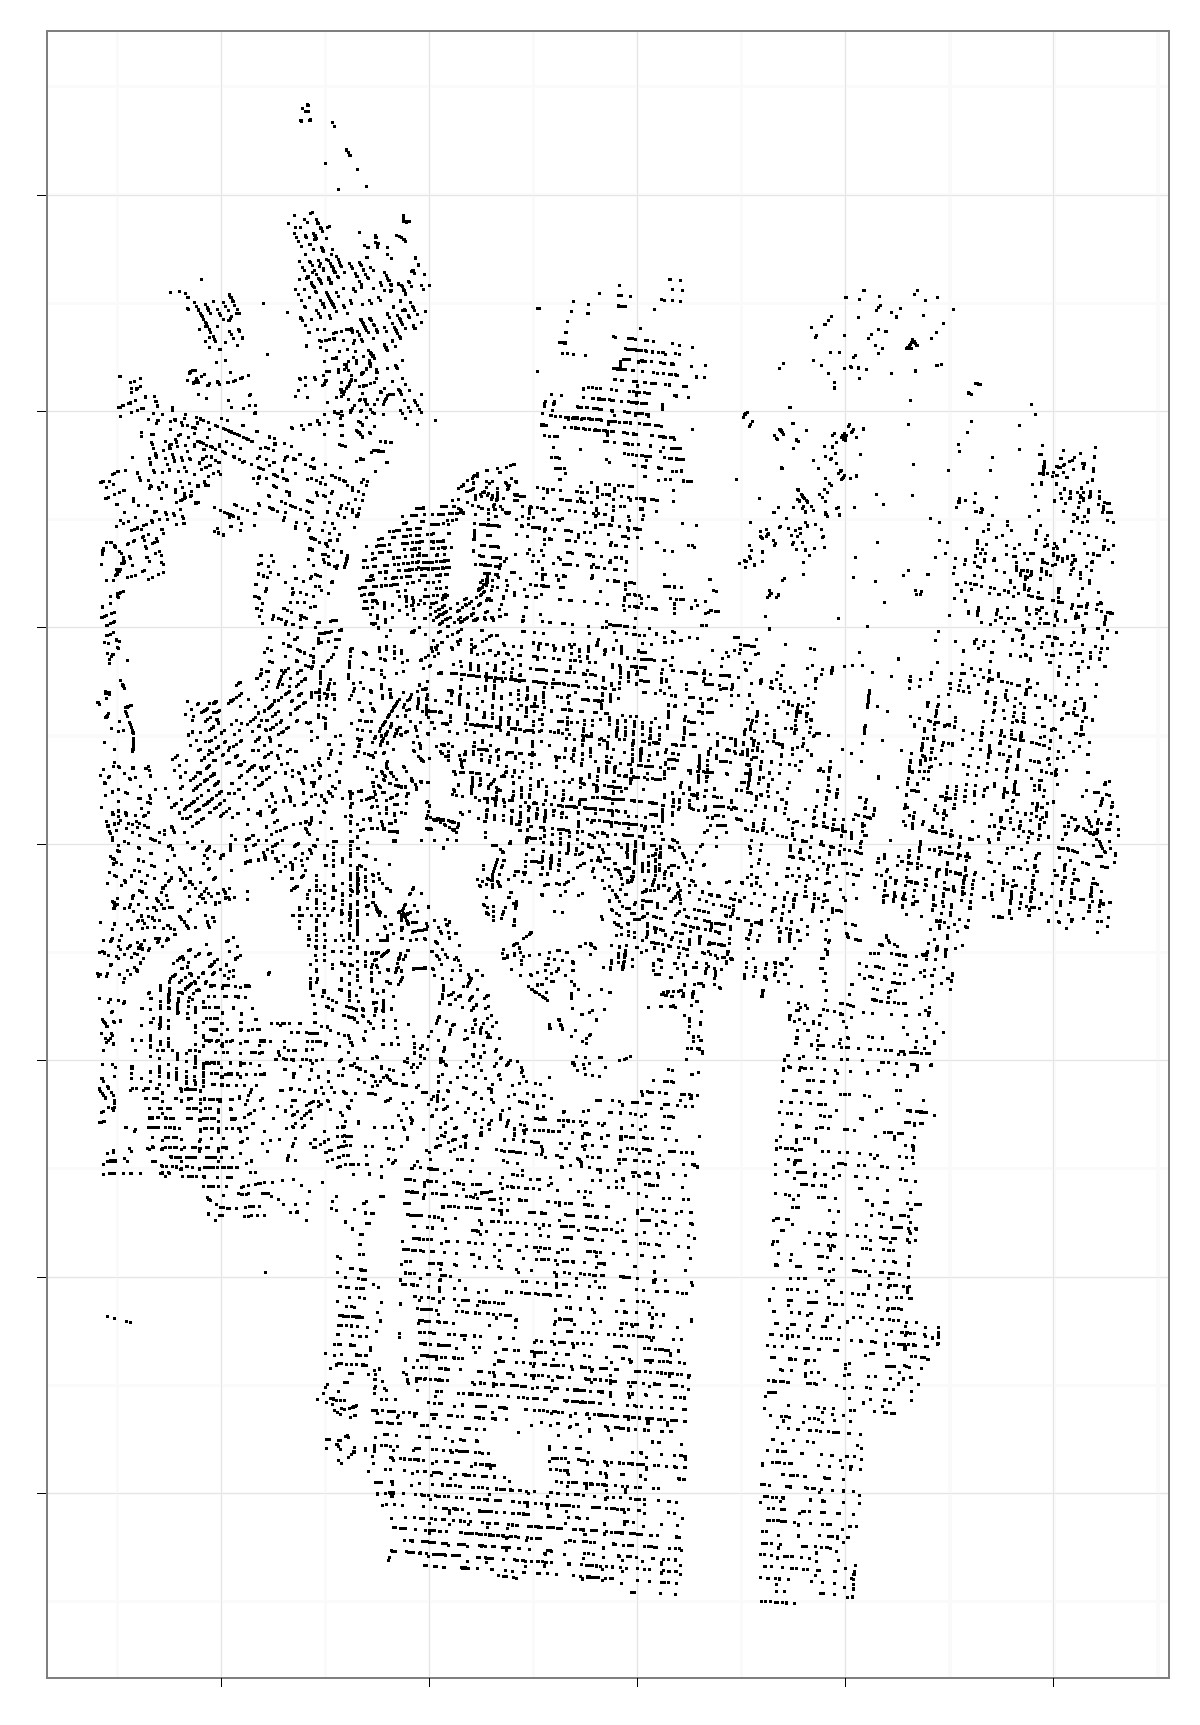
\includegraphics[width=0.9\linewidth]{sf-geo-big}
%   \caption{}
%   \label{fig:sf-big}
% \end{figure}


% We can also use this data for an unexpected purpose.  Because the data is so dense and includes the year that the house was built, we can explore historical patterns of housing development.  This idea was inspired by truliaHindsight, \url{http://hindsight.trulia.com/}, but because we have the data in an unencumbered form we are much freer to experiment with the visualisation of this data.  They have much more data, 150,000 vs 27,000, but we can display more (they display at most 2000 points at once), and we can do more sophisticated analyses.

\section{Conclusions}

All the tools we use are open source: you can download them and replicate our work yourselves.  The principle of reproducible research (cite Gentleman and Temple Lang) paper is very important for science - we provide enough detail that you can follow out work every step of the way, and you can run a script to reproduce exactly what we did.  A little tricky because working on this data analysis also lead us to develop some new tools, and it takes some time for these to trickle into released versions.  If you have problems running the code we released, please let us know!  Data analysis like software development.  Local caches to speed things up and to provide some backup if the original sources go down.

Tension with interactive tools: they are great for discovery, but bad for reproducibility.  Once you have discovered something in your interactive tool, you need to be able to reproduce it independently so that others can see it too.  Area of active research (cite Heer's work).  Also need to note your findings as you go along - no way to do this purely in code.  If you read the code on the website you'll see we've used comments to note down what we see and the analysis follows a fairly logical flow.  This is different to what happens in practice - there are many blind alleys that didn't make the final cut.  We rely on the rcs system to keep these, although currently lacking tools to easily search past versions and see the wrong paths that we went down.

Tools: shell (wget, awk); R (ggplot2, plyr, reshape).

Note about graphics: can churn out rough versions for exploration very quickly - takes more time to polish them for publication.  Clarify story, remove extraneous elements and ensure that it supports the text.


% bibtool -x beautiful-data.aux > references.bib
\bibliography{references}

\end{document}
